
\chapter{Architektura}


\section{System oznaczania zębów}
W tym rozdziale opisano budowę aplikacji. Ważną częścią jest opis sposobu komunikacji między komponentami aplikacji oraz zestawienie modeli danych. Aplikacja jest złożona z~kilku komponentów:
\begin{itemize}
\item Klient
\item Serwer
\item Baza danych
\end{itemize}
Do każdego komponentu użyto innej technologii. W~celu zaimplementowania klienta użyto języka JavaScript oraz frameworka Vue. Do zbudowania serwera skorzystano z~języka Python i~mikroframeworka Flask. Baza danych jest na podstawie technologii MongoDB, czyli systemu bazodanowego typu NoSQL lub inaczej, nierelacyjnego.

Architektura aplikacji tego modułu w~ogólności jest architekturą typu klient-serwer.\cite{clientServer} Typ charakteryzuje się tym, że wielu użytkowników za pomocą klienta może korzystać z~serwisów udostępnianych przez serwer. Klient jest rodzajem aplikacji lub procesu, który wysyła oraz odbiera wiadomości od serwera. Przykładem klienta jest aplikacja uruchamiana w~przeglądarce pod danym adresem internetowym. Taki rodzaj klienta użyty jest w~module systemu oznaczania zębów.

\begin{figure}[ht!]
\centering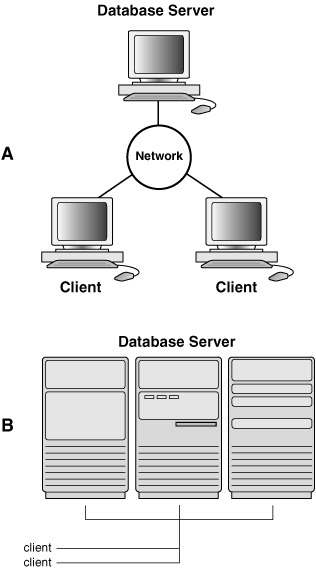
\includegraphics[width=75mm,scale=1.5]{figures/clientServerStanfor.jpg}
\caption{Przykładowy diagram budowy aplikacji, z~serwerem bazodanowym, o~architekturze klient-serwer.\cite{clientServerStanford}}
\label{fig:clientServerStanford}
\end{figure}

Dokładny sposób działania architektury klient-serwer jest następujący. Serwer jest serwisem uruchomionym w~trybie ciągłym. Serwer oczekuje na przyjęcie żądania od klienta. Po otrzymaniu żądania opracowuje odpowiedź i~zwraca ją klientowi. W~ogólności serwer zapewnia wykonanie wszystkich specyficznych i~złożonych operacji, aby aplikacja klienta nie była zależna od skomplikowanych wymagań sprzętowych i~oprogramowania. Serwer wystawiony w~sieci internetowej, fizycznie znajduje się w~zaawansowanej maszynie o~dużej mocy obliczeniowej. Natomiast użytkownik korzystający z~klienta, często operuje prostym komputerem osobistym bądź nawet urządzeniem mobilnym typu smartphone. Ważnym aspektem, który zachęca do używania architektury klient-serwer jest scentralizowanie dostępu do innych systemów poprzez serwer. Oznacza to, że klient nie musi mieć dostępu bezpośredniego do, przykładowo, baz danych. Cała komunikacja z~bazą danych jest poprowadzona przez serwer, który zapewnia prędkość i~bezpieczeństwo dostępu. Od aplikacji klienckiej wymagane będzie tylko uwierzytelnienie prawa dostępu do danej usługi prezentowanej przez serwer. Kolejnym istotnym aspektem jest dostęp do serwer przez wiele klientów na raz. Klienty mają możliwość w~sposób symultaniczny korzystać z~serwisów dostarczanych przez serwer. Aspekt ten wymaga od serwera dodatkowych systemów obsługi wielu zapytań od wielu klientów. Dzięki czemu klient może być prostszą i~zajmującą mniej miejsca pamięci aplikacją.


\subsection{Budowa aplikacji}
Architektura modułu, system oznaczania zębów, różni się od klasycznej architektury klient-serwer. Różnicą jest, że w~obecnej wersji oprogramowania pełna funkcjonalność działa tylko na lokalnej maszynie. Oznacza to, że serwer musi być uruchomiony na tej samej maszynie co klient. Jest to związane z~przetwarzaniem komend głosowych oraz urządzeń zewnętrznych potrzebnych do tego procesu. Nie zmieniają się inne zalety architektury klient-serwer. Nadal istnieje możliwość, w~obrębie maszyny z~serwerem, uruchomić kilka klientów i~działać na nich symultanicznie. Baza danych, nie musi być uruchomiona na tej samej maszynie. Aczkolwiek domyślne ustawienia łączności oczekują, że adres bazy będzie lokalny.

Komunikacja między komponentami odbywa się przy użyciu protokołu HTTP. Jest on często wykorzystywany podczas budowy aplikacji typu REST API. Moduł systemu oznaczania zębów jest zbudowany w~oparciu o~REST ale w~obecnej wersji nie spełnia wszystkich jego zasad. Styl REST odwołuje się do programistycznego interfejsu aplikacji, który spełnia opisane zasady architektury oraz pozawala na interakcję z~webowymi serwisami typu RESTful.\cite{restapibook} Akronim API oznacza zbiór definicji i~protokołów do budowania i~integracji aplikacji. Natomiast REST to zbiór ograniczeń i~zasad architektonicznych, nie jest to konkretny protokół lub standard. Deweloperzy zajmujący budową API, mogą w~wiele sposobów zaimplementować REST.

Działanie aplikacji typu REST jest proste i~pozwala na łatwe monitorowanie komunikacji. Kiedy żądanie klienta jest zrealizowane przez RESTful API, jest ono przekazywane razem z~treścią do węzła końcowego.\cite{restapi} Węzły końcowe są standardowo zlokalizowane na serwerze. Informacje przekazywane w~żądaniu są dostarczane w~postaci jednego z~kilku podstawowych formatów. Przykładowo formatami takimi są:
\begin{itemize}
    \item JSON
    \item HTML
    \item XML
\end{itemize}
Obecnie najczęściej używanym formatem jest JSON. Jego dużą zaletą jest czytelność plików, która pozwala zrozumieć zawartość osobom bez wiedzy technicznej. Istotną częścią żądania są nagłówki oraz parametry, które określa się metadanymi. Zawierają informacje takie jak: dane do autoryzacji, dane ciasteczek, pamięć podręczną, URI, kod statusu połączenia oraz inne dane.

Określenie konkretnej aplikacji typem RESTful\cite{restapibook}, wymaga od niej spełnienia kryteriów:
\begin{itemize}
    \item Architektura klient serwer - pozwala na odseparowanie interfejsu użytkownika od przechowywania danych. Pozwala na zwiększenie możliwości przenoszenia i~uruchamiania klienta na różnych platformach. Poprawia również skalowalność, upraszczając komponenty serwera.
    \item Bezstanowość - bezstanowa komunikacja klient-serwer oznacza, że żadne dane o~kliencie nie są przechowywane przez serwer między żądaniami. Zapewnia, że każde żądanie jest oddzielne i~niezależne od innych.
    \item Pamięć podręczna - buforowanie dostarczonych przez żądania danych po stronie klienta. Składowanie takich danych ma na celu zwiększenie prędkości przetwarzania żądań poprzez powtórne użytkowanie wcześniej zdobytych danych. Ustawienia tego procesu powinny mieć na uwadze, że część otrzymywanych danych może się różnić, nawet w~dwóch żądaniach do tego samego węzła końcowego na serwerze.
    \item System warstwowy - organizowanie każdego typu serwera, np. odpowiedzialnego za bezpieczeństwo czy równoważenie obciążenia, w~warstwy połączone ze sobą. Takie podejście pozwala na dużą skalowalności aplikacji. Klient komunikujący się, z~tak zbudowanym serwerem, nie jest w~stanie określić z~jaką warstwą jest aktualnie połączony.
    \item Jednolity interfejs - zastosowanie dokładnie określonego API pozwala na separację implementacji klient i~serwera. Styl REST podaje bardziej techniczne uwagi na temat budowania takiego interfejsu:
    \begin{itemize}
        \item Na podstawie pojedynczego żądania, serwer jest w~stanie zidentyfikować użytkownika. Standardowo w~tym celu umieszcza się w~wiadomości adres URI.
        \item Klient może manipulować otrzymanymi zasobami za pośrednictwem reprezentacji. Ponieważ reprezentacja zawiera wystarczającą ilość informacji, aby to zrobić.
        \item Wiadomości zwracane do klienta zawierają wystarczającą ilość informacji, aby opisać, jak klient powinien je przetwarzać. Przykładem jest ustawianie pola metadanych o~typie zawartości w~nagłówku żądania HTTP. Dla formatu JSON, pole to jest powinno być ustawione na 	,,application/json''.
        \item Dostępny jest hipertekst lub hipermedia. Po uzyskaniu dostępu do zasobu klient powinien mieć możliwość korzystania z~hiperłączy, w~celu znalezienia wszystkich dostępnych działań, które może wykonać. 
    \end{itemize}
    \item Kod na żądanie - wysyłanie kodu wykonywalnego z~serwera do klienta na żądanie. Pozwala na rozszerzenie funkcjonalność klienta. Ten punkt jest opcjonalny przy budowie aplikacji typu REST.
\end{itemize}

Budowa aplikacji modułu systemu oznaczania zębów spełnia część z~podanych wyżej kryteriów. Jest oparta na architekturze klient-serwer. Występuje komunikacja bezstanowa. Aplikacja jest za mała aby w~pełni korzystać z~systemu warstwowego, ale oddzielnie działa baza danych i~API do rozpoznawania mowy. Spełnione jest też założenie jednolitego interfejsu. Nie jest zaimplementowana możliwość korzystania z~kodu na żądanie. Pamięć podręczna nie jest w~pełni kontrolowana przez napisane oprogramowanie. 


\begin{figure}[ht!]
\centering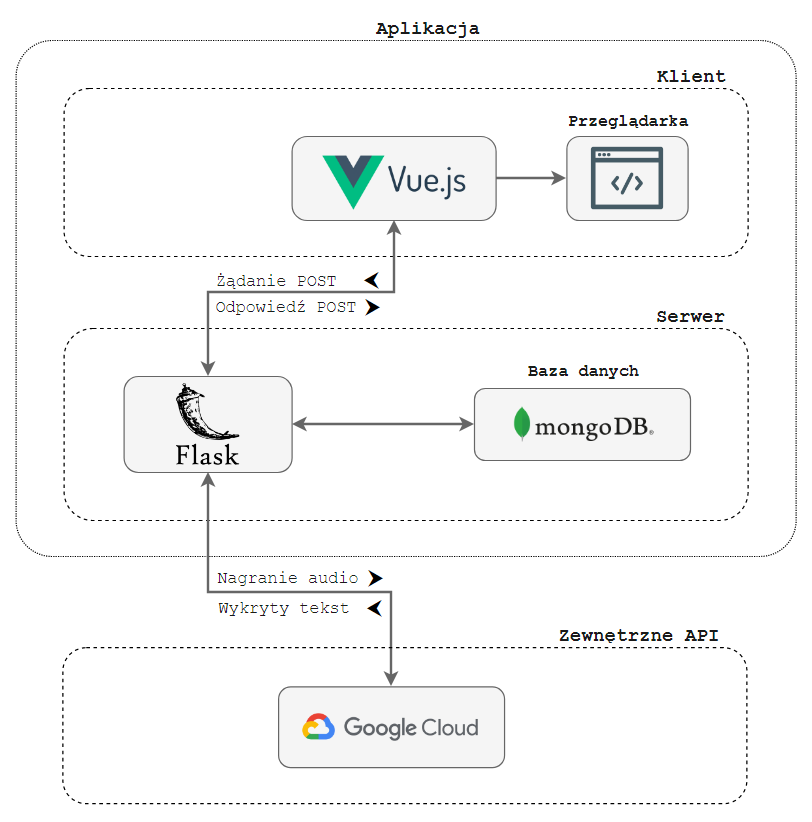
\includegraphics[width=140mm,scale=1.5]{figures/app.png}
\caption{Diagram budowy aplikacji modułu - system oznaczanie zębów.}
\label{fig:appArch}
\end{figure}

Na diagramie z~rysunku \ref{fig:appArch} jest przedstawiona budowa aplikacji oraz przepływy danych. Głównym komponentem jest serwer zrealizowany w~technologii Flask. Odpowiada on za obsługę żądań od klientów. Komunikacja odbywa się za pomocą żądań HTTP. Sposób budowy aplikacji jest oparty o~styl REST, którego szczegóły zostały opisane wcześniej.


Od strony serwera, za komunikację odpowiadają węzły końcowe. Każdy z~węzłów ma inny adres, w~celu  unikalności. Przykładowy węzeł końcowy, w~technologii Flask i~języku Python, podano poniżej:
\begin{lstlisting}
@app.route('/getPersonData', methods=['POST'])
\end{lstlisting}
Zakładając, że serwer uruchomiony jest na adresie 127.0.0.1, oraz że przyjmuje standardowy dla Flask port 5000. Pełnym adresem dla tego węzła jest:
\begin{lstlisting}
127.0.0.1:5000/getPersonData
\end{lstlisting}
W przykładzie widać również, że jest podane jakiego typu metoda HTTP obsługuje węzeł. W~tym module, w~prawie całej komunikacji, używana jest metoda POST. Nazwy węzłów zwyczajowo opisują operację wykonywaną przez serwis węzła. W~przykładzie taką operacją będzie pobranie danych osoby z~bazy danych i~dostarczenie ich, w~wiadomości zwrotnej, do klienta. 

Zgodnie z~diagramem z~rysunku \ref{fig:appArch}, komunikację w~aplikacji można podzielić na 3 kanały. Pierwszym kanałem jest połączenie serwera Flask z~klientem. Klient jest aplikacją uruchomioną na porcie 8080 w~przeglądarce internetowej. Jest to najważniejszy kanał komunikacji, ponieważ obsługuje żądania klienta. Na podstawie tych żądań wywoływanych jest większość operacji w~aplikacji. Serwer i~klient wymieniają między sobą wiadomości zawierające dane osób, które są pacjentami stomatologicznymi. Dokładny opis wiadomości znajduję się poniżej w~podrozdziale ,,Modele danych''. Drugim kanałem jest połączenie serwera Flask i~serwera bazy danych. Baza przechowuje dane pacjentów oraz parametry dotyczące chorób i~części zębów. Połączenie używane jest do dostarczania i~zapisywania danych na żądania klienta. Używane jest także przy komponowaniu komend z~tekstu otrzymanego z~interfejsu rozpoznawania mowy. Trzeci kanał jest między serwerem Flask a~zewnętrznym API. Połączenie to wymaga dostępu do internetu. Google Speech Recognition API przyjmuje na wejście plik audio nagrany poprzez mikrofon użytkownika. Plik zostaje przetworzony na tekst i~wysłany jako odpowiedź do serwera aplikacji. Jeżeli komenda zostanie uznana za poprawną, Flask przesyła ją do klienta. Frontend zrealizowany w~technologii Vue jest asynchroniczny, dzięki czemu zmiana wywołana komendą jest natychmiast widoczna w~przeglądarce internetowej. Zmiana nie jest w~tym momencie zapisana do bazy danych. W~celu zapisu nowych danych należy posłużyć się odpowiednim przyciskiem na widoku danych osobowych. 

\subsection{Modele danych}
W aplikacji modułu systemu oznaczania zębów dane przechowywane są nierelacyjnej bazie danych w~technologii MongoDB. Dane w~bazie zapisane są w~formacie JSON. JSON to format wymiany danych. \cite{json} Charakteryzuje się, tym że zawiera małą ilość pamięci danych, oraz że jest prosty do czytania i~tworzenia dla ludzi. Dodatkowo jest łatwy do przetwarzania i~generowania dla maszyn. Jako format tekstowy jest w~pełni niezależny od konkretnego języka programowania. Aczkolwiek jego konwencja bazuje na językach z~rodziny C, taki jak C, C++, Java czy Python. Wszystkie te właściwości sprawiają, że JSON jest dobrym językiem wymiany danych. 
\begin{figure}[ht!]
\centering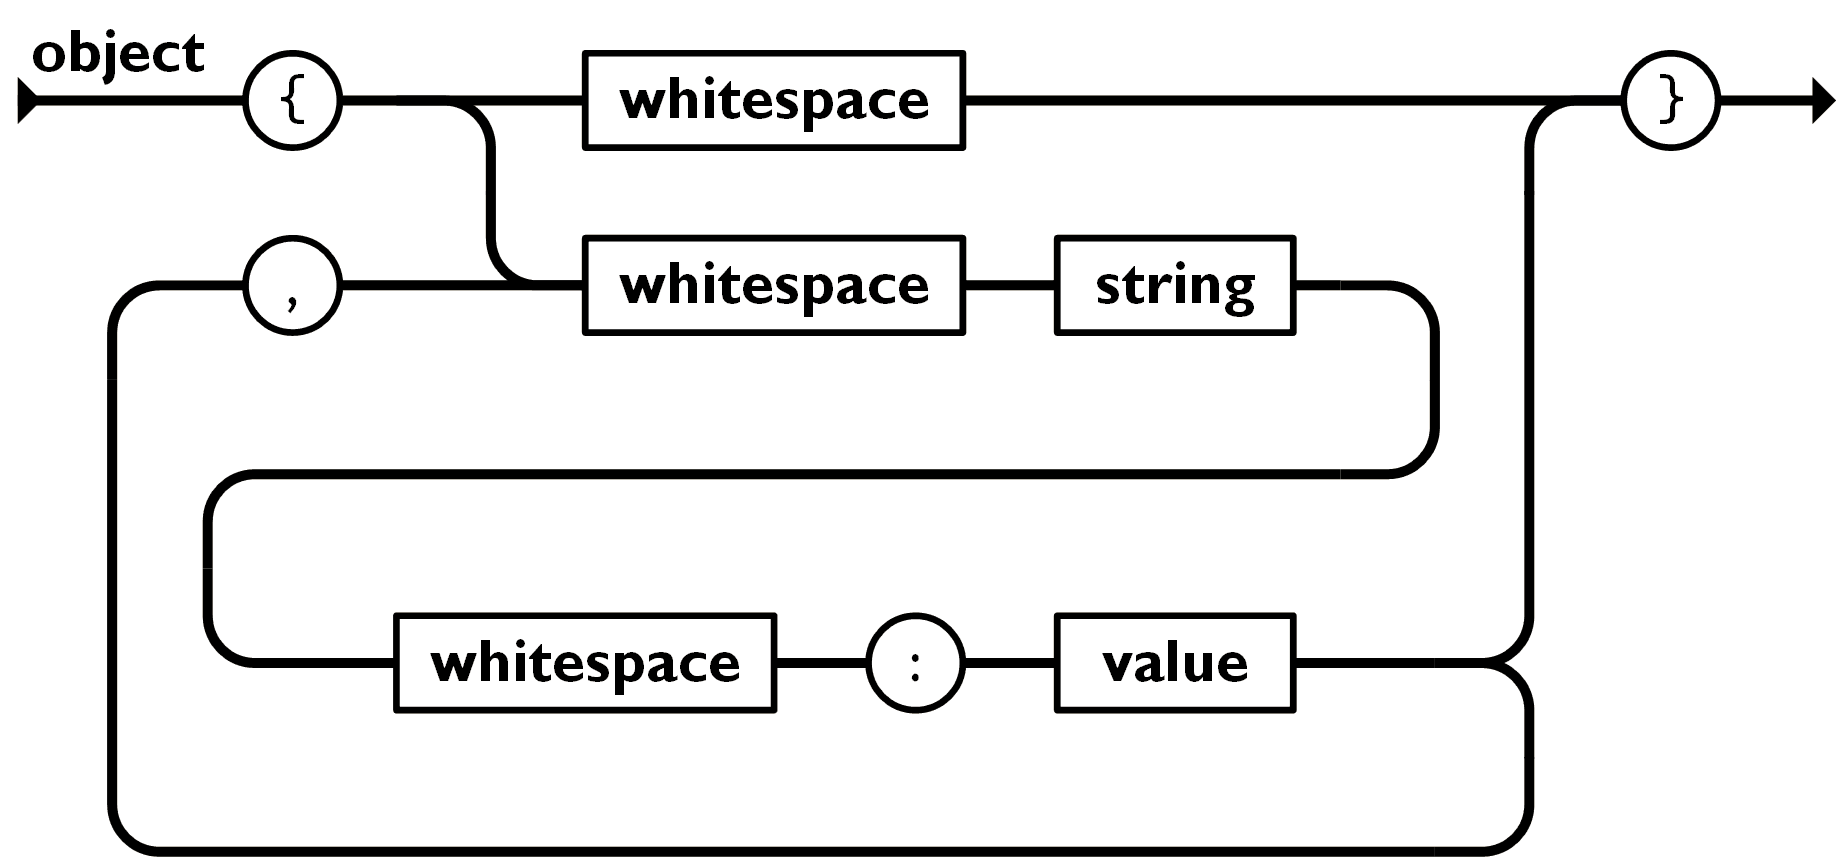
\includegraphics[width=145mm,scale=1.5]{figures/json1.png}
\caption{Diagram budowy podstawowego obiektu w~formacie JSON.}
\label{fig:jsonBuild}
\end{figure}
Diagram budowy obiektu w~formacie JSON jest zaprezentowany na rysunku \ref{fig:jsonBuild}. Dane zapisywane są przy pomocy klucza i~wartości oddzielonych dwukropkiem. Przykładem obiektu mogą być dane osobowe zawierające imię, nazwisko oraz PESEL. Taki obiekt prezentował by się w~formacie JSON jak poniżej.
\begin{lstlisting}
    {
        "imie" : "Jan",
        "nazwisko" : "Kowalski",
        "PESEL" : "87101912345"
    }
\end{lstlisting}
Format pozwala na prezentowanie bardziej skomplikowanych struktur, jak tablice obiektów:
\begin{lstlisting}
    "klienci" : [
        {
        "imie" : "Wojciech",
        "nazwisko" : "Sosnowski",
        "PESEL" : "87101912346"
        },
        {
        "imie" : "Krzysztof",
        "nazwisko" : "Tan",
        "PESEL" : "87101912347"
        }
    ]
\end{lstlisting}

Baza danych zawiera dwie kolekcje. Pierwszą jest ,,customers'', która zawiera wszystkie dane o~pacjentach. Dokument składa się z~czterech głównych obiektów:
    \begin{itemize}
        \item PersonalDetails - zawierający pola: imię, drugie imię, nazwisko, data urodzenia, PESEL, płeć
        \item ContactDetails - zwierający pola: numer telefonu, adres poczty elektronicznej oraz adres zamieszkania podzielony na nazwę ulicy, numer budynku, numer skrzynki pocztowej, kod pocztowy i~miasto 
        \item PermanentTeeth - zawiera dane 32 zębów stałych
        \item PrimaryTeeth - zawiera dane 20 zębów mlecznych
    \end{itemize}
Dodatkowo każdy dokument posiada pole daty wersji. Jest ono używane przy obsłudze wersji danych. Proces ten opisany jest w~dalszej części pracy. 
Ząb również jest obiektem. Technicznie, od strony programistycznej, ząb mleczny oraz ząb stały, są takim samymi obiektami. Ząb zawiera 5 pól. Każde z~pól oznacza jedną powierzchnię zęba. Nazwa powierzchni jest kluczem, a~wartością jest nazwa choroby. Dla powierzchni zdrowych, wartością jest wartość pusta, czyli ,,null''. Nazwy powierzchni są zakodowane jako wielkie litery, od A do E. Takie rozwiązanie jest podyktowane terminologią stomatologiczną, która dla tych samych powierzchni ma różne nazwy dla różnych zębów. Dla przykładu ząb o~numerze 11 ma powierzchnie sieczną, natomiast powierzchnia zęba o~numerze 15, na tej samej płaszczyźnie, to powierzchnia żująca. 
\begin{figure}[ht!]
\centering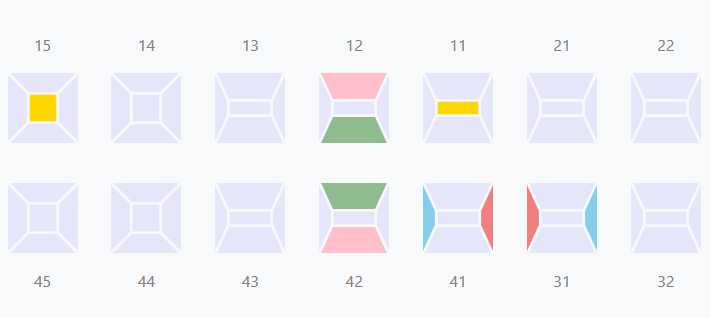
\includegraphics[width=145mm,scale=1.5]{figures/zeby.PNG}
\caption{Wycinek diagramu zębowego z~aplikacji.}
\label{fig:zeby}
\end{figure}
Na rysunku \ref{fig:zeby} kolorem żółtym oznaczono podany przykład. Innymi kolorami niż żółty, oznaczono powierzchnie, które mają takie same nazwy. Obrazuje to, że nazwa powierzchni zależy też od umiejscowienia zęba. Podobny problem jest z~terminologią chorób, które mają wiele nazw. Zaimplementowane rozwiązanie zostało dokładnie opisane w~rozdziale piątym, w~podpunkcie o~trudnościach oraz testowaniu.

Drugą kolekcją w~bazie danych, jest kolekcja ,,parameters''. Dokumenty zapisane w~niej, mają różne modele danych. Zawierają parametry i~słowniki. Pierwszy dokument zwiera słownik chorób. Oznacza to, że jeżeli choroba ma trzy nazwy, to jedna nazwa jest główna. Dwie pozostałe zostaną przetłumaczone na nazwę główną w~celu ujednolicenia nazw chorób na serwerze i~przy kolorowaniu diagramu zębowego. Tłumaczenie dotyczy tylko serwera. Dla użytkownika aplikacji oznacza to, że wypowiadając komendę głosową, może używać różnych nazw, tej samej choroby. Dla przykładu, ,,most'', ,,implant'' i~,,proteza'' oznaczane są takim samym kolorem na diagramie zębowym. W~celu uproszczenia komunikacji między serwerem a~klientem, wszystkie te nazwy tłumaczone są na słowo ,,proteza''. Poniżej zaprezentowano jak wygląda tłumaczenie w~formacie JSON dla podanego przykładu.
\begin{lstlisting}
    {
        "translation" : "most",
        "desease" : "proteza"
    }, 
    {
        "translation" : "implant",
        "desease" : "proteza"
    }, 
    {
        "translation" : "proteza",
        "desease" : "proteza"
    }
\end{lstlisting}
Drugi dokument zawiera analogiczny słownik dla nazw powierzchni zębów. Problem nazewnictwa powierzchni został opisany wcześniej oraz jest poruszony w~rozdziale piąty, w~temacie testowania aplikacji.
Kolekcja ,,parameters'' w~założeniu może być edytowana przez programy zewnętrzne, w~celu np. dodania translacji. W~związku z~tym, kolekcja ta jest aktualizowana przy każdy uruchomieniu serwera Flask.

Jak wspomniano wcześniej, w~dokumentach kolekcji ,,customers'' jest dodatkowe pole - data wersji. Jest to pole używane do procesu wersjonowania. Data, a~dokładniej czas, jest rejestrowany z~dokładnością do milisekund. Pozwala to na zapis kilku wersji tego samego dnia. Założeniem tego procesu w~aplikacji jest możliwość prześledzenia zmian na diagramie zębowym przez użytkownika aplikacji. Wersjonowanie dotyczy całych dokumentów. Każda nowa wersja jest nowym dokumentem. Nowa wersja powstaje po użyciu przycisku ,,Zapisz dane'' na widoku danych osobowych. Wersje można przeglądać na widoku diagramu zębowego. Data wersji jest jednym z~dwóch pól, które użyto do wyszukiwania dokumentów w~kolekcji ,,customers''. Drugim polem jest PESEL, który pozwala na zidentyfikowanie unikalnego pacjenta. Ze zbioru dokumentów z~tym samym numerem PESEL, jest wybierany na podstawie daty wersji np. najnowszy. W~związku, z~użytkowaniem pola PESEL do wyszukiwania, jest ono wymagane przy zapisie. Na polach PESEL, imię, nazwisko ustawione walidacje, które nie pozawalają utworzyć nowej wersji, bez ich wypełnienia. Reszta pól, czyli też wszystkie pola kontaktowe, jest opcjonalna i~nie blokuje zapisu.

\section{Analiza odchylenia toru odwodzenia żuchwy}
Polecam zrobić taki diagram jak u mnie, nawet jak będzie miałe dwa okienka, to zabiera dużo miejsca :)

W tej sekcji przedstawiono logiczną organizację modułów aplikacji mierzącej dewiację zgryzu. Następnie omówiono poszczególne etapy procesu analizy nagrań.

\subsection{Proces analizy nagrań}

Analizę, której poddawane jest nagranie można podzielić na trzy podzadania:
\begin{itemize}
    \item detekcję szczęk,
    \item śledzenie wykrytych szczęk w kolejnych klatkach,
    \item pomiar odchylenia na podstawie położenia szczęk.
\end{itemize}
Każdy kolejny etap korzysta z wyniku etapu poprzedniego, niezależnie od wewnętrznej logiki działania. Możliwe zatem było zaimplementowanie ich jako osobnych modułów o dość znacznej autonomii. W dalszej części rozdziału znajduje się opis działania każdego z nich.

\subsection{Etapy detekcji szczęk pacjenta}

Detekcja zębów na klatkach nagrania przebiega w sposób wielostopniowy: początkowe przekształcenia intensywności poszczególnych pikseli służą wyodrębnieniu regionów zainteresowania, z których wybierane są te najbardziej zgodne z kryteriami modelującymi pożądane cechy. Prostokątne obszary będące wyjściem modułu detekcji ostatecznie zyskują w logice aplikacji wyższego poziomu semantyczną interpretację  szczęk pacjenta. Poniżej omówiono szczegóły każdego etapu pracy detektora.

Nagrania wczytywane z pliku domyślnie reprezentowane są przez bibliotekę OpenCV w przestrzeni barw BGR \cite{opencv_colors}. Istotnym utrudnieniem w rozpoznawaniu obiektów na obrazach jest zmienność oświetlenia, która w reprezentacji BGR wpływa na wszystkie trzy składowe pikseli. Aby w łatwiejszy sposób operować na kolorach będących 'immanentną' cechą obiektów, obraz przekształcany jest w przestrzeń kolorów HSV, w której jasność (V -- \emph{value}) rozpatrywana jest niezależnie od odcienia (H -- \emph{hue}) i nasycenia koloru (S -- \emph{saturation}).  

Z wstępnego oglądu przekazanych nagrań wynika, że rozkład każdej z trzech składowych kolorystycznych obrazu nie zawiera podziału na wyraźne klasy. W istocie, wartości pikseli należących do zębów pacjenta pokrywają się z tymi odpowiadającymi skórze lub przyrządom dentystycznym. Z tych względów na etapie początkowej segmentacji wykorzystywany jest fakt, że w większości przypadków widoczne są dziąsła otaczające pożądany obszar zębów. Zatem progowanie eliminujące piksele o wyraźnie dominującym odcieniu czerwonym umożliwia podział obrazu na rozłączne obszary zębów oraz reszty twarzy \ref{fig:threshold}.

\begin{figure}
    \centering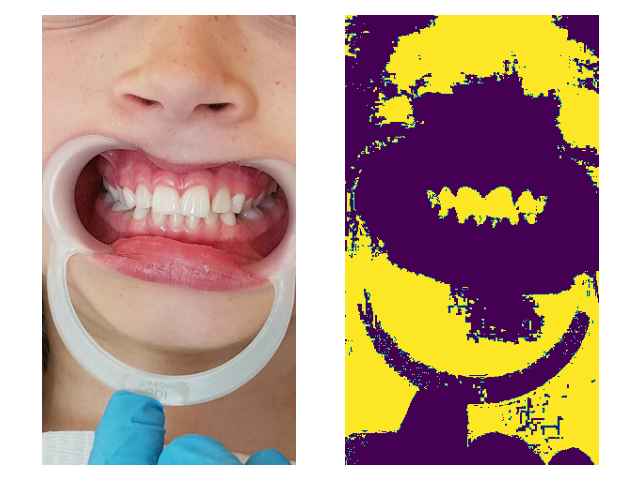
\includegraphics[width=75mm,scale=1.5]{figures/threshold.png}
    \caption{Progowanie obrazu według wartości odcienia}
    \label{fig:threshold}
\end{figure}

Po wykorzystaniu informacji zawartych w rozkładzie kolorów otrzymywana jest maska binarna zawierająca regiony potencjalnie będące szczękami, które na dalszym etapie poddawane są analizie z skupionej na kształcie i położeniu.  

Na etapie definiowania kryteriów, niestety, konieczne było poczynienie założeń w kwestii rotacji oraz skali obiektów na nagraniach, co ogranicza ogólną skuteczność detektora, jednak nie w przypadku nagrań dostarczonych na etapie rozwoju oprogramowania.  
Kroki procesu eliminacji potencjalnych regionów przedstawione są na rysunku \ref{fig:selection}. Najpierw (kolumna a), z maski usuwane są regiony o powierzchni przekraczającej maksymalną wartość,  przylegające do krawędzi obrazu (warunek rozmiaru jest konieczny, ponieważ może zdarzyć się, że fragment szczęki wykroczy poza zakres klatki). Następnie eliminowane są segmenty zbyt małe, aby uznać je za regiony odpowiednie do śledzenia (b). Pozostałe fragmenty oceniane są ze względu na wypukłość (\emph{solidity}), będącą stosunkiem pola obszaru do pola jego otoczki wypukłej \cite{regionprops}. Ponieważ zęby ukazane w sposób frontalny stanowią zwarty, wypukły kształt, wykluczone zostają regiony zbyt wklęsłe (c). W kolejnym kroku badana jest orientacja segmentów (d), czyli stosunek krótszej osi obrazu do osi wielkiej elipsy odpowiadającej badanemu segmentowi \cite{regionprops}; pozostawiane są tylko regiony o wystarczająco niskiej wartości tego kąta. Ostatnim etapem selekcji jest odrzucenie regionów oddalonych od środka nagrania.

\begin{figure}
    \centering 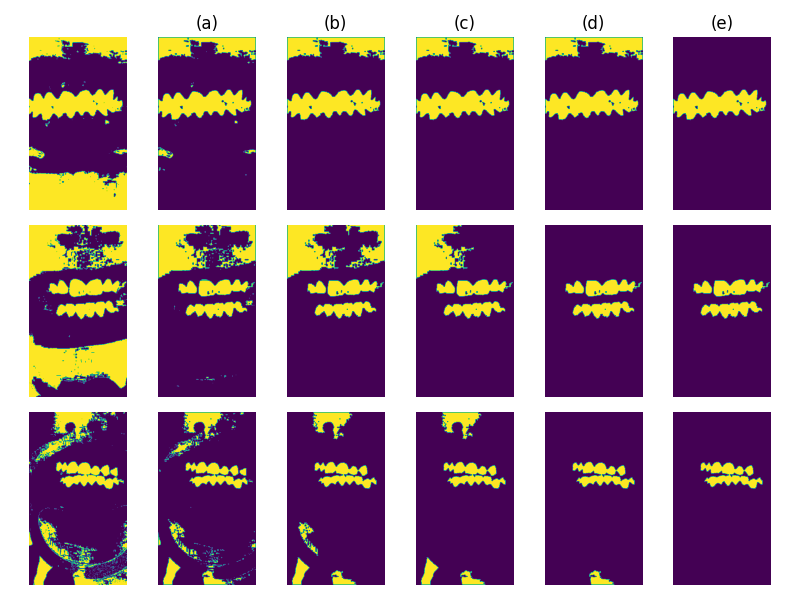
\includegraphics[width=140mm]{figures/selection.png}
    \caption{Rezultaty selekcji potencjalnych regionów na podstawie: (a) maksymalnego rozmiaru i przylegania do krawędzi, (b) minimalnego rozmiaru, (c) wypukłości, (d) orientacji, (e) odległości od środka}
    \label{fig:selection}
\end{figure}

Ostatnią kwestią objętą przez algorytm detekcji są sytuacje stykania się szczęk. Przetwarzanie omówione do tego momentu pozostawia zamknięte szczęki jako jeden region, co oczywiście uniemożliwia odpowiednie śledzenie ich ruchu. Z tego powodu przeprowadzana jest procedura wykrycia linii mogących stanowić krawędzie sieczne szczęk i podziału regionu wzdłuż owych linii. Wymienione poniżej etapy tego procesu zostały zilustrowane na rysunku \ref{fig:line_split}.

Na początku stosowany jest filtr Sobela, mierzący gradient intensywności pikseli wzdłuż twarzy (\ref{fig:line_split} a), co powoduje wyeksponowanie prostopadłych krawędzi (tj. punktów o odpowiednio wysokiej wartości gradientu). Z otrzymanego obrazu następnie otrzymywane są współrzędne linii wykrytych za pomocą transformacji Hougha (b). Znalezione odcinki muszą spełniać kryteria minimalnej długości i maksymalnej przerwy pomiędzy pikselami, dlatego możliwe jest, że na regionie nie zostaną wykryte odpowiednio wyraźne linie i przetwarzanie zakończy się. W przeciwnym wypadku spośród znalezionych odcinków wybierany jest ten, którego środek znajduje się najbliżej środka regionu, ale nie dalej niż 25\% odległości do krawędzi. Ostatecznie, obszar dzielony jest wzdłuż otrzymanej linii (c).

\begin{figure}
    \centering 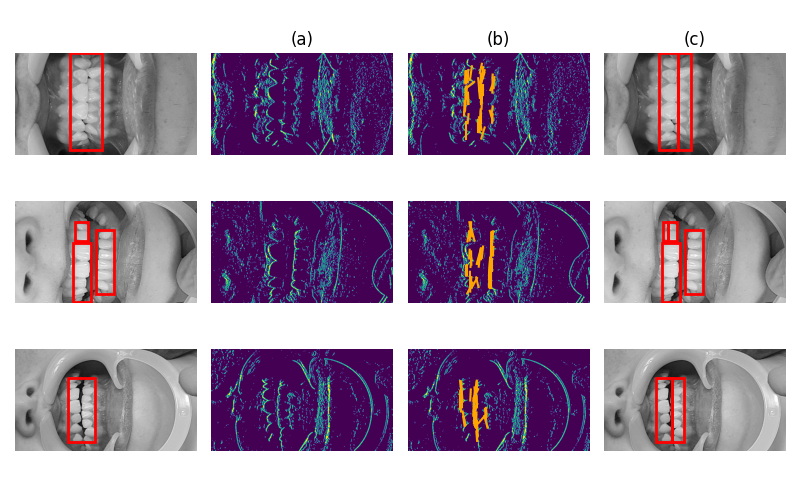
\includegraphics[width=140mm]{figures/line_split.png}
    \caption{Etapy podziału regionów: (a) wykrywanie krawędzi, (b) wykrywanie linii, (c) otrzymane nowe regiony}
    \label{fig:line_split}
\end{figure}

\subsection{Śledzenie szczęk}

Z formalnego punktu widzenia śledzenie oraz detekcja dostarczają odpowiedzi na to samo pytanie: Które piksele nagrania należą do obiektu będącego przedmiotem zainteresowania, a które nie? Faktycznie, w niektórych zastosowaniach dla każdej klatki wykorzystuje się jeden, ten sam algorytm detekcji, oznacza to jednak pominięcie informacji możliwej do uzyskania z poprzednich obserwacji. Poprawę wydajności, a nierzadko również skuteczności, przynosi zastosowanie algorytmu przewidującego trajektorię obiektu na podstawie informacji o jego położeniu w poprzednich klatkach, czyli trackera. W aplikacji zastosowano podejście, w którym śledzenie i detekcja wzajemnie się uzupełniają, czego szczegóły omówiono poniżej.  

Rdzeniem procesu śledzenia jest implementacja algorytmu MedianFlow dostarczona w bibliotece OpenCV \cite{opencv_trackingAPI}. Twórcy biblioteki zadbali o zapewnienie wspólnego interfejsu każdemu z oferowanych trackerów. Zatem to, który dokładnie algorytm wykorzystywany jest przez aplikację może zostać bardzo łatwo poddane modyfikacji, dzięki zastosowaniu wzorca projektowego strategii. Taka, oparta na technice wstrzykiwania zależności, architektura pozwoliła na sprawdzenie skuteczności wielu dostępnych algorytmów śledzenia bez konieczności zmiany pozostałego kodu.  

Poza samym aktualizowaniem trackera, przeprowadzana jest również walidacja zwracanych przez niego trajektorii szczęk. Powszechnym problemem takich algorytmów jest stopniowe "gubienie" śledzonego regionu, zwykle powodowane zmianą jego wyglądu lub widoczności. Z tego powodu, w regularnych odstępach czasu uruchamiana jest ponowna detekcja szczęk, której wynik następnie porównywany jest z regionami aktualnie wskazywanymi przez tracker. Miarą jakości wykorzystywaną w tej ocenie jest korelacja histogramów regionów odpowiadających szczękom. Jeśli wynik nowej detekcji cechuje się istotnie wyższą wartością tego kryterium oraz któryś z nowo znalezionych obszarów nie pokrywa się z żadnym z poprzednich w więcej niż 40\%, to aktualizowana jest para śledzonych regionów. Można taką sytuację interpretować jako utratę przez algorytm śledzenia trajektorii którejś ze szczęk.

\subsection{Pomiar dewiacji}

Po ustaleniu położenia szczęk, ostatnim etapem analizy jest obliczenie odchylenia dolnej szczęki względem pionowej trajektorii ruchu.